\documentclass{article}
\usepackage[parfill]{parskip}
\usepackage[a4paper, total={6in, 9in}]{geometry}

\usepackage{titlesec}
\titlespacing*{\section}{0pt}{0.01\baselineskip}{0.01\baselineskip}

\usepackage{graphicx} %Paquete para incluir imagenes

\titleformat{\paragraph}
{\normalfont\normalsize\bfseries}{\theparagraph}{1em}{}
\titlespacing*{\paragraph}
{0pt}{3.25ex plus 1ex minus .2ex}{1.5ex plus .2ex}


\graphicspath{ {./images/} }
%\usepackage[margin=1cm]{geometry} % Centra el texto

\begin{document}

\begin{titlepage}
  \vspace*{1cm}

  \begin{center}
    {\Huge{Informe del Trabajo Practico 1}}
  \end{center}

  \vspace{0.4cm}

  \begin{center}
    {\LARGE{Facultad de Ingeniería de la Universidad de Buenos Aires}}\\
    \vspace{0.3cm}
  \end{center}

  \vspace{0.8cm}
  \begin{center}
    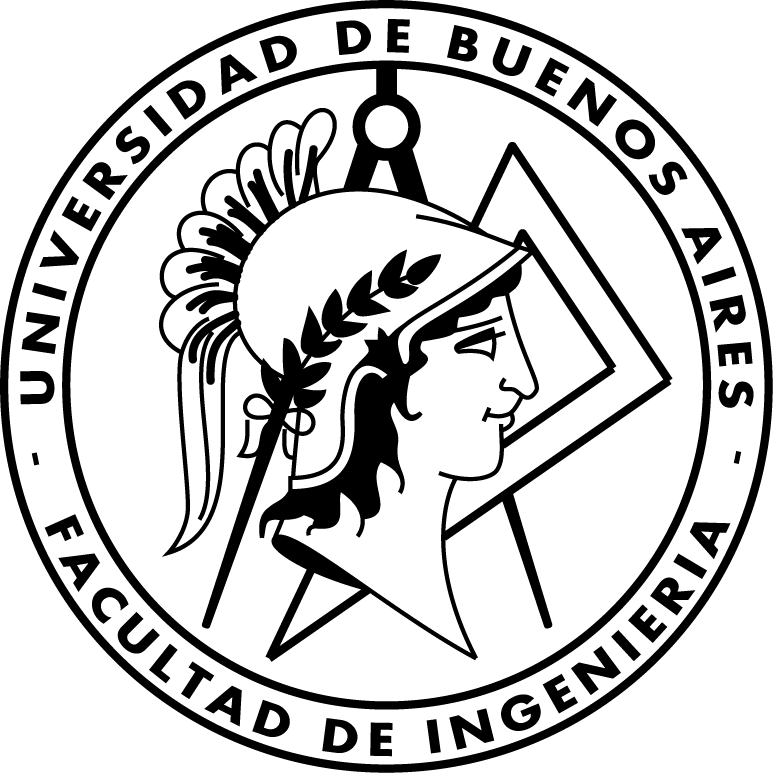
\includegraphics[scale=0.8]{Logo-fiuba}
  \end{center}

  \vspace{0.4cm}
  \begin{center}
    {\Large{Grupo 09}}\\
    \vspace{0.6cm}
    {\begin{minipage}[t]{.32\textwidth}
        \begin{center}
	Castro  Martinez, Jose Ignacio\\
          {\small{Padrón: 106957}}\\
          {\small{email: jacastrom@fi.uba.ar}}
        \end{center}
	\end{minipage}
	\begin{minipage}[t]{.32\textwidth}
        \begin{center}
	Douce, German Alejandro\\
          {\small{Padrón: 106001}}\\
          {\small{email: gdouce@fi.uba.ar}}\\
        \end{center}
      \end{minipage}
      \begin{minipage}[t]{.32\textwidth}
        \begin{center}
          Orsi, Tomas Fabrizio\\
          {\small{Padrón: 109735}}\\
          {\small{email: torsi@fi.uba.ar}}
        \end{center}
      \end{minipage}}
  \end{center}
\end{titlepage}


\section*{Preprocesamiento}

Antes de crear modelos predictivos se realizó un breve análisis exploratorio manual del Dataset (espiando el csv mano) y descubrimos que había algunas reseñas en inglés. Procedimos a eliminarlas y creamos un nuevo Dataset sin ellas. Este filtro no fue un 100\% efectivo ya que fue hecho a mano y con palabras elegidas por nosotros pero consideramos que fue logró eliminar la mayoría de las reviews en inglés sin eliminar muchas en español. En base a este dataset se trabajó con todos los modelos. En la red neuronal, además de esto, se quitaron las stopwords.
En cuanto a la vectorización utilizamos Tdif vectorizer pero su búsqueda de hiperparametros fue realizada junto con cada uno de los modelos que lo necesitaban (Naïve-Bayes, Random Forest y XGboost). Para la red neuronal hicimos Bag of Words a mano leyéndolo del libro de la cátedra (ver dicha sección).

\section*{Naive - bayes}

Una vez estudiado la generación del modelo base y de observar sus métricas realizamos una búsqueda de hiperparametros considerando la mayor cantidad de hiperparametros tanto para el modelo de predicción como el vectorizador, teniendo como hiperparametros del modelo:
alpha, fit prior y class prior. Por otro lado, también se realizó búsqueda de hiperparametros en el vectorizador, buscando de manera aleatoria los mejores valores posibles y probando con la mayor cantidad posible de datos, tales como: stopwords, frecuencia de aparición de palabras minimas y maximas, y número de ngramas. 

Una vez entrenado el modelo con los mejores hiperparametros, se obtiene un F1-score de aproximadamente 0.77, se le hizo validación cruzada con el propósito de verificar que actuara bien y no estuviese sesgado ante una clase particular y se generó una predicción para kaggle 

\section*{Random forest}
Para este modelo, decidimos setearle al Random Forest los parametros min\_samples\_leafs (15),  min\_samples\_splits (40) y n\_estimators (40) porque luego de hacer algunas pruebas vimos que los valores por default de estos generaban modelos gigantescos y cuya precision no mejoraba significativamente respecto a otros más chicos. Con este modelos obtuvimos una precision, recall y f1\_score de 0,83 con el conjunto de test local. En kaggle obtuvimos un puntaje de 0,698.
Luego, realizamos una optimización haciendo una búsqueda con GridSearch pero obtuvimos resultados un poco desconcertantes. La precisión, recall, y f1\_score bajaron a 0,81 en el conjunto de test local y en kaggle el puntaje bajó 4 puntos  a 0,65. 

Los hiperparametros recomendados por Grid search para el random forest (puntualmente) no variaron respecto a los que habíamos utilizado en el primer modelo. Esto se debe a que Grid Search suele optar por los menores valores para estos con el objetivo de evitar el Overfitting. 
En cuanto a los hiperparametros del vectorizador, recomienda no usar stopwords (las de la lista de la librería NLTK que mandamos como parámetro), no quitar acentos, y usar como analyzer: "word". La principal diferencia es en cuanto al minimo y maximo numero de palabras a tener en cuenta para armar el vocabulario. Recomienda eliminar las palabras que representan menos del 1\% del vocabulario y aquellas que representan más del 10\% del vocabulario. Creemos que esto último es lo que nos hace disminuir un poco el puntaje en Kaggle y las métricas.

Como conclusión de este modelo podemos decir que la búsqueda de hiperparámetros permite encontrar un modelo más simple y menos pesado con la esperanza de que generalize mejor y no Overfitte a la vez que no disminuye en gran medida el valor de las métricas. 
Sin embargo, reconocemos que algo no está del todo bien ya que lo esperado en la materia es que el modelo optimizado performe -por lo menos- igual de bien (o mal) que el no optimizado. En nuestro caso, como ya dijimos, una posible causa que puede estar causando esto es el hiper parámetro “mx\_df”  que es un valor bastante bajo (10\% del vocabulario) y que puede estar generando en el modelo una disminución muy importante de la performance al recortar en gran medida el mismo.


\section*{Xg boost}

Para el XGBoost realizamos un proceso similar a los modelos anteriores: entrenamos un modelo base para observar el comportamiento estándar del modelo y posteriormente se realiza la búsqueda de hiperparametros para intentar mejorar el modelo. 

En un principio se buscaron conjuntos de hiperparámetros para el modelo y para el vectorizador solo uso de stopwords. Este modelo es el que más se tardó en entrenar pero posee una mejor precisión en su métrica F1. 

Por otro lado, se hizo un esfuerzo extra por buscar hiperparametros agregando hiperparametros al vectorizador, pero dichos esfuerzos no fueron suficientes puesto que los modelos entrenados no tuvieron buen rendimiento en la predicción de sentimientos


\section*{Red neuronal}
En el caso de la red neuronal, seguimos el diseño que recomendaba la bibliografía\footnote{Hands-on Machine Learning with Scikit-Learn, Keras \& TensorFlow por Aurélien Géron}.
Para esto poder usar la red neuronal tuvimos que tokenizar el texto. Para esto contamos la aparición de cada una de las palabras del set de entrenamiento y las ordenamos en una lista según su frecuencia. Cada palabra tenía como ID su posición en dicha lista. Decidimos ponerle un límite a la cantidad de palabras del vocabulario, ya que, según el libro, esto no disminuiría la eficacia.  Luego tokenizamos los textos (train, test y de submit), transformando cada palabra por su índice de la tabla anterior. 
Para la red neuronal, empezamos con una layer de embedding, la cual convierte los tokens a vectores. Luego, usamos la layer intermedia “GRU”, siguiendo la guía del libro. Esta tiene un comportamiento muy similar a la LSTM. Las “GRU”, según lo que conversamos en clase,  son óptimas para el análisis de sentimiento, con el beneficio de tener una mayor performance. Finalmente un layer “denso” con un único output que determina si la review fue positiva o negativa. 
Con esta red neuronal “básica”, hicimos una predicción sobre el set de submit. Sus métricas fueron: accuracy: 0.85,  Recall: 0.80, Precisión: 0.89, f1 score: 0.85. Esta predicción nos dio muy malos resultados (43\%).
Para mejorar estos resultados. decidimos hacer una búsqueda de hiper parámetros.  Para esto, hicimos un random search de distintos parámetros (Cantidad de layers densas, cantidad de épocas, función de activación de dichas layers, tamaño del batch). Luego de obtener los hiperparametros, construimos la red neuronal. Esta nueva red tuvo una mejora considerable con respecto al modelo anterior. Sus métricas fueron: accuracy: 0.8, Recall: 0.91, Precisión: 0.76, f1 score: 0.83. Sin embargo, tuvo un acierto del 48\%; siendo este nuestro peor modelo. 


\section*{Ensamble - voting}


Para el ensamble híbrido, optamos por armar un modelo híbrido de tipo voting que utiliza alguno de los modelos anteriormente entrenados (un Naive Bayes, un XgBoost y un Random Forest) Armamos el modelo y posteriormente realizamos la validación cruzada del mismo para comprobar su comportamiento y que no desmejore las métricas anteriormente obtenidas por cada modelo individualmente. Este modelo resultó ser uno de los mejores modelos a la hora de predecir y analizar las emociones del texto 

Nota: El modelo con la mejor predicción de kaggle fue un ensamble voting que no cumplía con los requisitos del enunciado puesto que este fue el resultado de la combinación del naives bayes con hiperparametros y el Xg boost (0,75). A pesar de todo, el ensamble híbrido que usa 3 modelos diferentes también es uno de los modelos con mejor predicción (0,72). 


\section*{Conclusiones}

El modelo con el que obtuvimos mejores resultados en Kaggle fue el Voting armado con 2 modelos ( NB + Xg boost) con un puntaje de 0,75 en Kaggle. Le sigue el Voting de 3 modelos (NB + Xg boost + RF) con un puntaje de 0,72. Esta diferencia se debe posiblemente a que el RF tuvo un performance bastante peor que los otros dos modelos. Por su parte, la superioridad del Voting se debe a la afamada frase “varios estimadores mediocres combinados puede crear una muy buena predicción.
En cuanto a los otros modelos, los resultados del mejor al peor en Kaggle fueron: Naive Bayes (0,71), Xg boost ( 0,70), Random Forest (0,65) y la red Neuronal (0,48).





\end{document}
